% MedBridge -- IEEE conference paper.
% GENERATED by report/paper/build_latex.py from report/paper/content/*.md and the results
% files of the repository. Rebuild instead of editing by hand (or stop regenerating once
% the team starts editing this file in Overleaf). Compile: pdflatex, bibtex, pdflatex x2.
% Red bold text (\pending{...}) marks placeholders and results that do not exist yet.
\documentclass[conference]{IEEEtran}
\IEEEoverridecommandlockouts
\usepackage[T1]{fontenc}
\usepackage[utf8]{inputenc}
\usepackage{cite}
\usepackage{amsmath,amssymb,amsfonts}
\usepackage{graphicx}
\usepackage{textcomp}
\usepackage{xcolor}
\usepackage{booktabs}
\usepackage{array}
\usepackage{tabularx}
\usepackage{listings}
\usepackage{algorithm}
\usepackage{url}
\DeclareRobustCommand{\pending}[1]{\textcolor{red}{\textbf{#1}}}
\lstset{basicstyle=\scriptsize\ttfamily, columns=fullflexible, keepspaces=true,
  breaklines=true, breakatwhitespace=false, frame=single, framesep=2pt,
  xleftmargin=3pt, xrightmargin=3pt, aboveskip=2pt, belowskip=0pt, upquote=true,
  showstringspaces=false}

\begin{document}

\title{MedBridge: A Dual Answerability Gate for Hallucination-Resistant Local Retrieval-Augmented Clinical Guidance}

\author{\IEEEauthorblockN{Vijay Aravindh S.}
\IEEEauthorblockA{\textit{\pending{[TO BE FILLED: department]}} \\
\pending{[TO BE FILLED: university]} \\
\pending{[TO BE FILLED: city]}, India \\
\pending{[TO BE FILLED: email]}}
\and
\IEEEauthorblockN{Mohammad Farhan Rashid}
\IEEEauthorblockA{\textit{\pending{[TO BE FILLED: department]}} \\
\pending{[TO BE FILLED: university]} \\
\pending{[TO BE FILLED: city]}, India \\
\pending{[TO BE FILLED: email]}}
\and
\IEEEauthorblockN{Maheswari S.}
\IEEEauthorblockA{\textit{\pending{[TO BE FILLED: department]}} \\
\pending{[TO BE FILLED: university]} \\
\pending{[TO BE FILLED: city]}, India \\
\pending{[TO BE FILLED: email]}}}

\maketitle

\begin{abstract}
Large language models explain clinical guidelines fluently, but in patient-facing cardiovascular care a fluent answer to a question the evidence does not cover is itself a safety risk, and a standard retrieval-augmented generation (RAG) pipeline answers every question it receives. We present MedBridge, a locally deployable assistant for hypertension and related cardiovascular care that makes answerability an explicit, auditable decision. A deterministic emergency fast-path screens each message before any model call. A Context Gate decides before retrieval whether missing personal facts call for a clarifying question, and an Evidence Gate decides after hybrid retrieval whether to answer, give general information, abstain or escalate. Abstentions and escalations are pre-vetted templates, so no generated text reaches the user on those paths. Two optional extensions can only make the system more conservative: a calibrated Evidence Gate with permutation voting, and a post-generation grounding verifier based on natural language inference. We introduce MedBridge-HalluBench, a synthetic benchmark of 247 conversations (298 turns) in six answerability categories, and compare the full system with direct-LLM, vanilla-RAG, prompt-only-safety and single-gate ablations, using a 4B-parameter open-weight model, an LLM judge and an NLI judge, and paired exact tests. \pending{[TO BE FILLED after the study: one or two sentences with the headline hallucination and unsafe-answer results, their confidence intervals and Holm-adjusted p-values, taken from evaluation/results/summary.json.]}
\end{abstract}

\begin{IEEEkeywords}
Retrieval-augmented generation, hallucination, abstention, clinical decision support, hypertension, large language models, patient safety
\end{IEEEkeywords}

\section{Introduction}\label{sec:intro}

Hypertension is a major and largely preventable driver of cardiovascular disease, yet many affected adults worldwide remain undiagnosed, untreated or uncontrolled \cite{who2023globalreport,ncdrisc2021hypertension}; in India, a national survey found it in roughly one adult in three \cite{anjana2023indiab}. Control depends on what patients understand between visits about their readings, medicines and lifestyle, and many now ask conversational AI. Large language models (LLMs) hold considerable clinical knowledge \cite{singhal2023llmclinical} but also produce confident statements that no source supports, usually called hallucinations \cite{ji2023survey}.

Retrieval-augmented generation (RAG) conditions the model on passages from a trusted corpus \cite{lewis2020rag} and has improved medical question answering \cite{xiong2024medrag}. A standard RAG pipeline, however, is built to answer whatever the quality of the match. Three routine situations in patient conversations defeat this design. A question can be answerable in principle while the safe answer depends on facts the patient has not given, such as a dose change for an unnamed medicine. A question can fall outside the evidence: a drug that does not exist, a false premise, a dose no guideline states, a topic outside cardiology. And a message can describe an emergency, where a long reply only delays care. Asking the generator to ``say when it does not know'' leaves the decision to the component most prone to over-confident output, although knowing when not to answer is a capability in its own right \cite{wen2025abstention}.

MedBridge instead makes answerability an explicit decision taken by separate components at fixed points around retrieval, each logged with its rationale. Deterministic rules handle emergencies before any model call. A \emph{Context Gate} (Gate 1) judges before retrieval whether the patient context suffices or a clarifying question is needed. An \emph{Evidence Gate} (Gate 2) judges after retrieval whether the passages support a specific answer, only general information, or nothing, and whether to escalate. Refusals and escalations never pass through the generator, and all models run locally, so no patient text leaves the device. Our contributions are:

\begin{enumerate}
\item the \emph{Dual Answerability Gate}, a five-action routing architecture (ANSWER, SOFT-ASK, GENERALIZE, ABSTAIN, ESCALATE) that separates missing \emph{context} from missing \emph{evidence}, with a deterministic emergency override and template bypass;
\item two strictly conservative extensions: a calibrated Evidence Gate and a post-generation grounding verifier (``Gate 3'');
\item MedBridge-HalluBench, a synthetic benchmark of casual, multi-turn patient questions labelled with the expected safe behaviour, and a calibration-gated evaluation protocol;
\item an open, fully local implementation sized for a 6 GB laptop GPU.
\end{enumerate}

Section~\ref{sec:related} reviews related work, Section~\ref{sec:method} presents the method and Section~\ref{sec:setup} the experimental setup. Section~\ref{sec:results} reports the results, Section~\ref{sec:discussion} discusses them, Section~\ref{sec:limitations} covers limitations and ethics, and Section~\ref{sec:conclusion} concludes.

\section{Related Work}\label{sec:related}

\textbf{Grounding and hallucination mitigation.} Beyond plain RAG \cite{lewis2020rag}, Self-RAG fine-tunes a generator to emit reflection tokens that decide when to retrieve and whether a segment is supported \cite{asai2024selfrag}, and Corrective RAG scores retrieved documents and refines or replaces them when confidence is low \cite{yan2024crag}. Other methods check text after it is written: Chain-of-Verification answers self-posed verification questions \cite{dhuliawala2024cove}, RARR retrieves evidence per claim and revises unsupported content \cite{gao2023rarr}, and SelfCheckGPT flags sentences that are inconsistent across samples \cite{manakul2023selfcheckgpt}. FActScore measures factual precision over atomic facts \cite{min2023factscore}. These approaches need a specially trained generator, still answer every input, or act only after generation. MedBridge decides \emph{before} generation whether an answer may be produced at all; its optional Gate 3 follows the post-hoc idea but can only delete content or withdraw the answer.

\textbf{Selective prediction and abstention.} Selective classification rejects inputs whose confidence falls below a threshold calibrated to bound the risk on accepted inputs \cite{geifman2017selective}, and a recent survey organises LLM abstention by query, model and human values \cite{wen2025abstention}. Such methods yield one answer-or-refuse signal. MedBridge separates two reasons not to answer that need different replies, missing personal context (ask) and insufficient evidence (generalise or abstain), and adds escalation; its calibrated variant borrows the selective-prediction idea for reranker scores.

\textbf{Evaluating medical LLMs.} Medical LLMs are mostly evaluated on exam-style multiple-choice sets that always require an answer \cite{singhal2023llmclinical,xiong2024medrag}; ours labels each turn with the expected behaviour, including asking, abstaining and escalating. We use an LLM judge \cite{zheng2023judging}, but because judges can favour their own model family \cite{panickssery2024llm}, it comes from a different family than the application model and is paired with a deterministic NLI judge.

\textbf{Patents and security.} Patented prior art includes a question-answering system that can return an explicit ``no answer'' \cite{bhagwat2017ibmnoanswer}, LLM detection of ambiguous queries followed by a clarifying question \cite{zhang2024intuitdisambiguity}, and RAG-based clinical decision support over a curated guideline library \cite{paul2025glasshealthrag}. In the documents we reviewed, none combines a pre-retrieval context gate, a post-retrieval evidence gate and a deterministic pre-model emergency override with template bypass. RAG applications are also exposed to prompt injection through user text and retrieved content \cite{greshake2023notwhat}, which motivates the input isolation in Section~\ref{sec:method}.

\section{The MedBridge Method}\label{sec:method}

MedBridge answers patient questions about hypertension and related cardiovascular topics (heart failure, atrial fibrillation, coronary disease, lipids, kidney- and diabetes-related blood pressure, pregnancy, lifestyle). It gives guideline-based information and never diagnoses or prescribes. Each turn passes through the pipeline of Fig.~\ref{fig:pipeline} (Algorithm~\ref{alg:routing}) and ends in one of five actions: ANSWER (a specific, cited answer), SOFT-ASK (a clarifying question), GENERALIZE (general guideline information, marked as such), ABSTAIN (a pre-vetted refusal) or ESCALATE (a pre-vetted emergency message).

\begin{figure}[t]
\centering
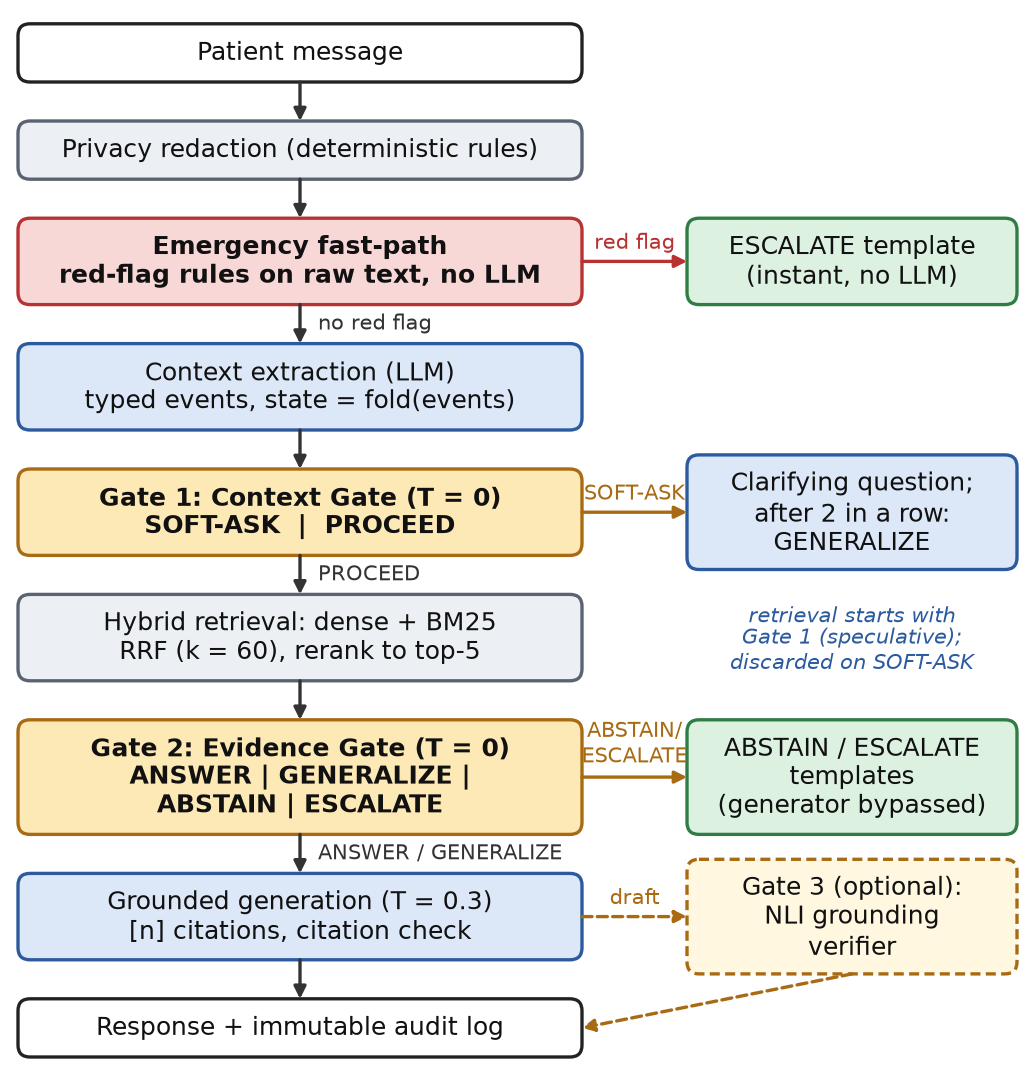
\includegraphics[width=0.94\columnwidth]{figures/gate_pipeline.png}
\caption{The MedBridge routing pipeline. Gates 1 and 2 are separate LLM decisions at temperature 0; emergency handling, refusals and escalations involve no generated text. Gate 3 is an optional extension (V2).}\label{fig:pipeline}
\end{figure}

\textbf{Design principles.} (i) Each answerability decision and its rationale go to an append-only audit log. (ii) Emergency triage, refusal and escalation texts, and the patient state are deterministic. (iii) LLM decisions are narrow classifications with JSON-schema outputs at temperature 0 and seed 42. (iv) Failures degrade safely: a failed extraction leaves the state unchanged, a failed Gate 1 defaults to PROCEED, a failed Gate 2 to GENERALIZE, and a failed generator to a pre-vetted template.

\subsection{Emergency Fast-Path and Patient State}

Before any model call, a rule-based classifier reads the raw message. It parses blood-pressure readings in many written forms and escalates at a systolic pressure of at least 180 mmHg or a diastolic pressure of at least 120 mmHg. The 2025 AHA/ACC guideline manages such severe hypertension as an outpatient matter when there is no acute organ damage \cite{jones2025aha}; a patient-facing tool cannot rule that out, so MedBridge deliberately escalates in this range. Further rules cover red-flag symptoms (chest pain, stroke signs, fainting, severe breathlessness), with clause-level filters for negation, informational questions and dated history, and normalisation of misspellings and Hinglish. Since nothing later can overrule it, this path favours recall over precision. For other messages, an extractor LLM converts the redacted text into typed delta events (reading, medication added or stopped, symptom, demographic, laboratory result), a search query and an intent summary. The LLM never writes the patient state: the snapshot is a deterministic fold over stored events, so one faulty extraction cannot overwrite earlier facts. Deterministic helpers map drug brands to generic names and expand lay terms for retrieval.

\subsection{Gate 1: Context Gate}

Gate 1 sees the snapshot and the message and returns PROCEED or SOFT-ASK with missing fields from a fixed vocabulary (current medicines, a recent reading, age, pregnancy status, ...). It may ask only when the question concerns the patient's own cardiovascular care, a specific personal fact would change the safe answer, and that fact is unknown. General, out-of-scope, fabricated, false-premise and otherwise unanswerable questions always proceed, because more context cannot make them answerable; Gate 2 handles them with the evidence. On SOFT-ASK the generator phrases a short question. A loop-breaker bounds the dialogue: if Gate 1 asks again after two consecutive clarifying questions, the turn is forced to GENERALIZE and Gate 2 is skipped.

\subsection{Hybrid Retrieval}

The knowledge base holds 27 open-access documents from 11 organisations, mainly clinical guidelines such as \cite{jones2025aha}, in 2,747 chunks of at most 400 tokens. Each query is encoded by a dense model (bge-small-en-v1.5 \cite{xiao2024cpack}) and by BM25; the two ranked lists are fused by reciprocal rank fusion with k = 60 \cite{cormack2009rrf}, and the top 20 candidates are reranked by a MiniLM cross-encoder \cite{nogueira2019passage} to the top 5. Retrieval depends only on the extractor's query, so it starts concurrently with Gate 1 and is discarded on SOFT-ASK, which leaves routing unchanged. On 70 labelled queries, fusion gave the highest mean reciprocal rank (0.740 [0.650, 0.825] against 0.677 [0.584, 0.766] for dense retrieval, 95\% bootstrap intervals), while reranking brought no measurable gain (nDCG@5 0.657 [0.569, 0.740] with, 0.688 [0.600, 0.771] without). We keep it because it is cheap and feeds V1.

\subsection{Gate 2: Evidence Gate}

Gate 2 sees the five chunks, the snapshot and the patient's own words and applies the first matching rule. ESCALATE: an emergency happening now that the fast-path missed. ABSTAIN: a question outside cardiovascular care; irrelevant or thin evidence; a named drug or product absent from the evidence (it may not exist); a dose or number the evidence does not state; paediatric or pregnancy medicine decisions the evidence does not cover. GENERALIZE: evidence that covers the topic only in general terms, or a false premise the evidence contradicts (the answer corrects it). ANSWER: evidence that addresses this question directly for this patient; when torn between ANSWER and GENERALIZE, the gate prefers GENERALIZE. A unit test checks that its few-shot examples share no topic or invented drug name with the benchmark.

\begin{algorithm}[t]
\caption{Routing of one patient turn in MedBridge}\label{alg:routing}
\begin{lstlisting}
input: raw message m; state S; consecutive SOFT-ASK count c
 1  r <- Redact(m)
 2  if EmergencyRules(m) fires: return Template(ESCALATE)
 3  (ev, q, intent) <- Extract(r, S);  S' <- Fold(S, ev)
 4  R <- start Retrieve(q)            # concurrent with Gate 1
 5  g <- ContextGate(S', r, intent)   # T = 0, seed 42
 6  if g = SOFT-ASK and c < 2:
 7      discard R; c <- c + 1; return Ask(g.missing)
 8  E <- top-5 Rerank(await R)        # dense+BM25, RRF k = 60
 9  if g = SOFT-ASK: a <- GENERALIZE; c <- 0   # loop-breaker
10  else: c <- 0; a <- EvidenceGate(E, S', r)  # T = 0
11  if a in {ABSTAIN, ESCALATE}: return Template(a)
12  d <- Generate(a, E, S', r)        # T = 0.3, [n] citations
13  if V2 enabled: (a, d) <- GroundingVerifier(a, d, E)
14  d <- ValidateCitations(d, E)
15  if a = ANSWER and d has no valid citation: a <- GENERALIZE
16  Persist(ev, turn, gate rationales) atomically; return (a, d)
\end{lstlisting}
\end{algorithm}

\subsection{Generation and Output Control}

For ANSWER and GENERALIZE a grounded generator (temperature 0.3) writes from the evidence only; every sentence stating a clinical fact must end with the index of its supporting chunk, and GENERALIZE answers must say that they give general information. A server-side check removes markers that point to no retrieved chunk, and an ANSWER left without a valid citation is downgraded to GENERALIZE. ABSTAIN and ESCALATE never reach the generator. In every prompt the patient's text sits in an \texttt{\textless{}untrusted\_\allowbreak{}user\_\allowbreak{}input\textgreater{}} element with tag-like sequences escaped, and the evidence in \texttt{\textless{}clinical\_\allowbreak{}evidence\textgreater{}}, as a defence against prompt injection.

\subsection{Optional Extensions V1 and V2}

Both variants keep the routing and can only make it more conservative. \textbf{V1 (calibrated Evidence Gate)} runs Gate 2 on three deterministic permutations of the evidence order, still at temperature 0, and takes the majority action, breaking ties towards the more conservative one. Thresholds on the top reranker score and on the share of the question's salient entities (drugs, numbers, clinical terms) found in the evidence can then lower ANSWER to GENERALIZE, or either to ABSTAIN, never the reverse. \textbf{V2 (``Gate 3'')} checks each claim sentence of a draft with an NLI cross-encoder against the chunks it cites. Unsupported sentences are removed while their share stays within a threshold $\tau$; above it, an ANSWER is regenerated as GENERALIZE and checked again, otherwise the ABSTAIN template is returned. Its NLI model differs from the evaluation's NLI judge. Thresholds of both variants are calibrated on the development split only.

\textbf{Implementation.} A FastAPI service keeps events and audit records in append-only PostgreSQL tables and retrieves from Qdrant; all models run locally through Ollama. Identifiers are redacted before any model call or write, and session data are encrypted with per-session keys whose destruction erases a session.

\section{Experimental Setup}\label{sec:setup}

We ask whether the Dual Answerability Gate reduces hallucinated and unsafe answers compared with LLM and RAG baselines, and what each gate contributes.

\subsection{MedBridge-HalluBench}

The benchmark contains 247 synthetic conversations with 298 patient turns, 43 of them multi-turn (Table~\ref{tab:hallubench_composition}); no real patient data are used. Most messages are casual (155 items); others use Indian English (35), typos (33) or clinical wording (24). Each category targets a safe behaviour: a cited answer for answerable items, a clarifying question first for items with missing context (some test the loop-breaker), general information for general topics, and abstention or correction for unanswerable in-domain items (fabricated drugs and treatments, false premises, doses or figures the guidelines do not state, paediatric and pregnancy questions). Out-of-domain items cover non-cardiac medicine and non-medical topics, and emergency items include colloquial red-flag descriptions. Each turn has a gold action and a set of acceptable actions (strict and lenient scoring), and notes name any fabricated entity or false premise. A stratified 20\% development split (seed 42; 49 conversations) is used only for model selection and calibration; results use the 198 test conversations.

\begin{table}[t]
\centering
\caption{Composition of MedBridge-HalluBench}\label{tab:hallubench_composition}
\footnotesize
\setlength{\tabcolsep}{4pt}
\begin{tabularx}{\columnwidth}{>{\raggedright\arraybackslash\hsize=1.78\hsize}Xcc>{\centering\arraybackslash\hsize=1.02\hsize}X>{\centering\arraybackslash\hsize=0.57\hsize}X>{\centering\arraybackslash\hsize=0.63\hsize}X}
\toprule
Category & Items & Turns & Multi-turn items & Dev items & Test items \\
\midrule
Answerable, complete context & 64 & 64 & 0 & 13 & 51 \\
Answerable, missing context & 40 & 88 & 40 & 8 & 32 \\
General topic & 31 & 31 & 0 & 6 & 25 \\
Unanswerable, in domain & 52 & 52 & 0 & 10 & 42 \\
Out of domain & 30 & 30 & 0 & 6 & 24 \\
Emergency & 30 & 33 & 3 & 6 & 24 \\
\midrule
Total & 247 & 298 & 43 & 49 & 198 \\
\bottomrule
\end{tabularx}
\par\vspace{2pt}{\scriptsize\itshape Source: evaluation/datasets/hallubench\_v1.json.\par}
\end{table}

\subsection{Conditions}

All conditions (Table~\ref{tab:conditions}) share the application model, corpus and retrieval stack and are selected through an internal switch that the public API does not expose. C2 adds to the vanilla RAG prompt a block that asks, in prose, for the behaviour the gates enforce. The reference C1G uses the production prompt without gates, so each gate's effect is measured against a baseline that differs from C3 to C5 only by the gates. The emergency fast-path is active everywhere except C0, so emergency items favour no gated condition. Identical LLM requests are computed once and cached under the model's content digest, so paired conditions differ only in pipeline structure; latency charges each cached call the median uncached latency of the same call.

\begin{table}[t]
\centering
\caption{Conditions compared in the study}\label{tab:conditions}
\footnotesize
\setlength{\tabcolsep}{4pt}
\begin{tabularx}{\columnwidth}{>{\raggedright\arraybackslash\hsize=1.06\hsize}Xcc>{\centering\arraybackslash\hsize=0.87\hsize}X>{\raggedright\arraybackslash\hsize=1.06\hsize}X}
\toprule
Condition & Retrieval & Gate 1 & Gate 2 & Generator prompt \\
\midrule
C0 Direct LLM & -- & -- & -- & no evidence \\
C1 Vanilla RAG & $\checkmark$ & -- & -- & answer from passages \\
C1G RAG reference & $\checkmark$ & -- & -- & production \\
C2 RAG + prompt safety & $\checkmark$ & -- & -- & vanilla + safety rules \\
C3 Context Gate only & $\checkmark$ & $\checkmark$ & -- & production \\
C4 Evidence Gate only & $\checkmark$ & -- & $\checkmark$ & production \\
C5 MedBridge & $\checkmark$ & $\checkmark$ & $\checkmark$ & production \\
V1, V2, V12 & $\checkmark$ & $\checkmark$ & $\checkmark$ (V1: calibrated) & production (+ Gate 3) \\
\bottomrule
\end{tabularx}
\end{table}

\subsection{Models}

One application model serves the extractor, both gates and the generator. It was chosen by running C5 on the development split with qwen3.5:4b, qwen3:8b \cite{yang2025qwen3} and gemma3:4b \cite{gemmateam2025gemma3}. On 59 turns, strict routing accuracy was 69.5\% [56.9, 79.7], 71.2\% [58.6, 81.2] and 40.7\% [29.1, 53.4] respectively (Wilson 95\% intervals), with median turn latencies of 10.3, 16.0 and 9.3 s. An exact McNemar test found no significant difference between the two Qwen models (8 against 9 discordant turns, p = 1.00), so we use qwen3.5:4b (4.2B parameters, Q4\_K\_M), which is faster and fits a 6 GB laptop GPU. Inference runs through Ollama on an Apple M5 machine with 24 GB of memory.

\subsection{Hallucination Judges}

The \emph{LLM judge}, gemma3:12b \cite{gemmateam2025gemma3}, is larger than the application model and from a different family; it runs at temperature 0 with structured output. It splits each response into atomic clinical claims \cite{min2023factscore}, leaving out greetings, questions and generic referral advice, and labels each claim SUPPORTED, UNSUPPORTED or CONTRADICTED under a strict rubric (only an explicit statement or a direct paraphrase counts). The evidence per claim is the condition's own chunks plus the top three chunks of an independent judge-side retrieval, so C0, which retrieves nothing, is judged on equal terms. It also classifies the behaviour and flags accepted false premises, endorsed fabricated entities and unsupported doses, never seeing the condition or category. The \emph{NLI judge} scores the same claims against the same passages with the cross-encoder nli-deberta-v3-base \cite{he2023debertav3}, taking the maximum entailment over three-sentence windows, with thresholds calibrated on the development split. Template responses contain no claims. A blinded, stratified 50-item sheet is prepared for human annotation.

\subsection{Metrics and Statistics}

The primary outcomes are the response-level hallucination rate (responses with at least one unsupported or contradicted claim) and the unsafe-answer rate on unanswerable items (a specific answer, a raised flag or an unsupported claim). Secondary outcomes include the unsupported-claim ratio, coverage and over-abstention on answerable items, routing accuracy, emergency recall, false escalation, citation precision and latency. The unit is the item-turn of the test split. Proportions carry Wilson 95\% intervals \cite{wilson1927probable}. C5 is compared with C0 to C4, and each variant with C5, by exact McNemar tests \cite{mcnemar1947note} with Holm correction within each family \cite{holm1979simple}; Cochran's Q tests C0 to C5 jointly \cite{cochran1950comparison}. Effect sizes are risk differences and odds ratios; judge agreement is Cohen's $\kappa$ \cite{cohen1960coefficient}. The protocol order is enforced in code: C5 is run and judged on the development split, thresholds are calibrated, and only then are all conditions run on the test split. Turns in which a component fell back to a default after an error are reported and excluded from headline metrics, and the analysis refuses headline results if they exceed 5\% of any condition's turns. Sensitivity analyses include those turns, drop 14 items worded like prompt examples, and repeat the tests per item.

\section{Results}\label{sec:results}

\noindent\pending{[PENDING: results.md]}

\section{Discussion}\label{sec:discussion}

\textbf{Why two gates.} The gates decide with different information at different times. Gate 1 sees only the conversation and the recorded facts, so it can ask for a missing medicine or reading before any evidence is fetched; Gate 2 sees the passages and can tell a well-covered question from one the guidelines do not answer. A single post-retrieval gate would treat ``I need to know your medicine'' and ``the guidelines do not say'' as the same failure, although they need different replies. C3 and C4 measure each gate against the C1G reference. \pending{[TO BE FILLED after the study: whether the ablation shows complementary contributions, citing the paired tests.]}

\textbf{Templates and coverage.} Serving ABSTAIN and ESCALATE from fixed texts removes generation, and with it hallucination, from the paths where an error costs most, and makes those replies easy to review clinically. The price is helpfulness when a gate abstains too readily, which is why coverage and over-abstention are reported beside the hallucination rates. \pending{[TO BE FILLED after the study: coverage cost of C5 relative to C1 and C2, and C5 against the prompt-only safety baseline C2.]}

\textbf{Small local models.} Each gate is a narrow classification with a JSON schema, which suits small local models: in model selection a 4B model routed no significantly worse than an 8B model and was faster. Every gate adds a model call; starting retrieval with Gate 1 hides part of that cost.

\textbf{Expected failure modes.} Gate 2 may accept related but non-specific evidence as sufficient (V1 targets this); the generator may add details beyond its cited passages after a correct ANSWER decision, which citation validation cannot catch (V2 targets this); and the fast-path escalates some benign messages that mention a red-flag symptom, a cost we accept for an unsupervised tool. \pending{[TO BE FILLED after the study: which failure mode dominated, with counts from evaluation/results/error\_analysis.md.]}

\section{Limitations and Ethics}\label{sec:limitations}

\textbf{Limitations.} The benchmark is synthetic: items, gold actions and notes were drafted by the team with the help of an AI assistant and have not yet been reviewed by clinicians, so the labels encode the authors' reading of the guidelines, and a few borderline items admit another defensible label. Its phrasing is author-approximated (one Hinglish item), and the line between answerable and unanswerable depends on the corpus at labelling time. Hallucination is measured by automatic judges: the local LLM judge is of moderate size (in development, a smaller judge changed a claim's label when the other claims in its batch changed), and the NLI judge is calibrated against it, so the two are not fully independent; agreement with human annotators is still to be measured. Results come from one application model, one judge and one hardware platform, and the paired tests treat turns of a conversation as independent, which the item-level analysis only partly addresses. The corpus is English and mainly international or Western, without an Indian national guideline. The emergency rules were developed on cases written by the same team, and the system has not been evaluated with patients.

\textbf{Ethics and privacy.} MedBridge is a research prototype for health information, not a medical device: it does not diagnose or prescribe, refers treatment decisions to the patient's doctor and directs suspected emergencies to emergency services. No human participants or real patient records were involved. \pending{[TO BE FILLED: institutional ethics statement, if the venue requires one.]} Inference stays on the local machine, identifiers are redacted before any model call or storage, conversations are encrypted per session, and erasure destroys the session key. Redaction is a safeguard, not a guarantee: on a blind held-out set its strict span recall was 0.744, so local-only processing remains the primary protection. These measures follow India's Digital Personal Data Protection Act \cite{dpdp2023india}. Grounding in current guidelines reduces, but does not remove, the risk of biased or outdated medical content.

\section{Conclusion}\label{sec:conclusion}

MedBridge treats answerability as a first-class decision in patient-facing clinical RAG: a deterministic emergency path, a pre-retrieval Context Gate and a post-retrieval Evidence Gate decide whether to answer, ask, generalise, abstain or escalate, and the riskiest outcomes involve no generated text. The system runs on local open-weight models sized for a laptop GPU and is evaluated on MedBridge-HalluBench with ablations, baselines, two judges and paired exact tests under a calibration-gated protocol. \pending{[TO BE FILLED after the study: the headline finding in one or two sentences, stated with the same caution as in Section V.]} Future work includes clinician review of the benchmark and templates, the human annotation, held-out evaluation of the emergency rules, Indian-language and Indian-guideline coverage, and a supervised pilot with patients.

\section*{Acknowledgment}

\pending{[TO BE FILLED: thanks to the department, institution and anyone who helped, and funding if any.]} Parts of the software, the benchmark items and the first draft of this manuscript were prepared with the help of an AI coding assistant (Claude, Anthropic). The authors reviewed, revised and take full responsibility for all content. \pending{[TO BE FILLED: check this disclosure against the AI-use policy of the chosen venue.]}

\bibliographystyle{IEEEtran}
\bibliography{references}

\end{document}
